\documentclass{article}

\usepackage{arxiv}

\usepackage[utf8]{inputenc} % allow utf-8 input
\usepackage[T1]{fontenc}    % use 8-bit T1 fonts
\usepackage{hyperref}       % hyperlinks
\usepackage{url}            % simple URL typesetting
\usepackage{booktabs}       % professional-quality tables
\usepackage[english]{babel}
\usepackage{nicefrac}       % compact symbols for 1/2, etc.
\usepackage{microtype}      % microtypography
\usepackage{graphicx}
\usepackage{stmaryrd}

\usepackage{amsthm}
\usepackage{amsfonts}
\usepackage{amsmath}
\usepackage{mathtools}

\usepackage{tikz}
\usetikzlibrary{angles,fit,arrows,calc,math,intersections,through,backgrounds}
\usepackage{qtree}

\usepackage{xstring}
\usepackage{wasysym}
\usepackage{textcomp}
\usepackage{blindtext}
\usepackage{subfiles}

\newtheorem{definition}{Definition}
\numberwithin{definition}{section}
\newtheorem{lemma}{Lemma}
\numberwithin{lemma}{section}
\newtheorem{proposition}{Proposition}
\numberwithin{proposition}{section}
\newtheorem{corollary}{Corollary}
\numberwithin{corollary}{section}
\newtheorem{theorem}{Theorem}
\numberwithin{theorem}{section}

\DeclareMathSymbol{\mathinvertedexclamationmark}{\mathclose}{operators}{'074}
\DeclareMathSymbol{\mathexclamationmark}{\mathclose}{operators}{'041}
\makeatletter
\newcommand{\raisedmathinvertedexclamationmark}{%
  \mathclose{\mathpalette\raised@mathinvertedexclamationmark\relax}%
}
\newcommand{\raised@mathinvertedexclamationmark}[2]{%
  \raisebox{\depth}{$\m@th#1\mathinvertedexclamationmark$}%
}
\begingroup\lccode`~=`! \lowercase{\endgroup
  \def~}{\@ifnextchar`{\raisedmathinvertedexclamationmark\@gobble}{\mathexclamationmark}}
\mathcode`!="8000
\makeatother

\newcommand{\intga}{\mathclap{\smash{\oplus}}{\int}}
\newcommand{\intgp}{\mathclap{\smash{\otimes}}{\int}}
\newcommand{\intgg}{\mathclap{\rightsquigarrow}\mathclap{\int}}

\DeclareMathOperator{\arcsinh}{arcsinh}
\DeclareMathOperator{\arctanh}{arctanh}

\title{Can arithmetic expressions form a geometry space?}

\date{}

\author{
Mingli Yuan \\
Swarma Research\\
Beijing, 100083 \\
\texttt{mingli.yuan@gmail.com}
}

% Uncomment to remove the date
%\date{}

% Uncomment to override  the `A preprint' in the header
\renewcommand{\headeright}{A preprint}
\renewcommand{\undertitle}{A preprint}

\begin{document}
\maketitle

\begin{abstract}
This study explores how arithmetic expressions can be systematically organized into geometric spaces.
By introducing a flow equation, we examine the processes—both infinitesimal and discrete—that transform arithmetic expressions into geometric structures.
Our investigation extends existing theoretical frameworks and provides concrete examples that conceptualize these spaces.
This research lays the foundation for future studies.
\end{abstract}

\keywords{arithmetic expressions, flow equation, arithmetic expression space}

\setcounter{tocdepth}{1}
\tableofcontents
\newpage

\section{Introduction}\label{sec:introduction}

The concept of systematically organizing arithmetic expressions into geometric spaces presents a compelling extension to traditional mathematical frameworks. Real numbers $\mathbb{R}$ can be conceptualized as a continuum of additive arithmetic expressions, while the exponential function over real numbers, $e^\mathbb{R}$, represents a continuum of multiplicative arithmetic expressions. This paper aims to extend these well-established ideas by characterizing and constructing geometric spaces formed by arithmetic expressions.

While the broader implications of AEG are vast, this paper focuses specifically on the definition and construction of AEG spaces.

\emph{Main Contributions}

The foundation of our approach lies in the introduction of a flow equation, which is critical for constructing the proposed geometric space. This flow equation describes the infinitesimal processes that generate arithmetic expressions, facilitating their transformation into neighboring forms. Our analysis demonstrates that this infinitesimal process is consistent with the discrete generation of arithmetic expressions at a specified granularity.

\emph{Structure of the Paper}

\begin{itemize}
    \item Section~\ref{sec:example}: presents an intuitive example that serves as context for the theoretical discussion.
    \item Section~\ref{sec:concepts}: outlines fundamental concepts to lay the groundwork for the detailed analyses that follow.
    \item Section~\ref{sec:flowequation}: discusses the flow equation, which is central to our theoretical framework.
    \item Section~\ref{sec:space}: elaborates on the general construction of an arithmetic expression space.
    \item Section~\ref{sec:conclusion}: synthesizes the findings and discusses directions for future research.
\end{itemize}

\section{An intuitive example}\label{sec:example}

Consider the upper half-plane $\mathcal{H} = \{(x, y) \mid y > 0\}$, equipped with an inner product and metric defined by:

\[
    \mathbf{a} \cdot \mathbf{b} = \begin{bmatrix} a_x & a_y \end{bmatrix} \begin{bmatrix} \frac{1}{y^2} & 0 \\ 0 & \frac{1}{y^2 \ln^2 2} \end{bmatrix} \begin{bmatrix} b_x \\ b_y \end{bmatrix}
\]

and

\[
    ds^2 = \frac{1}{y^2} (dx^2 + \frac{dy^2}{\ln^2 2})
\]

In this setting, we introduce a scalar field $a$, which is defined by the following relationship:

\begin{equation}
    a = - \frac{x}{y}\label{eq:assignment}
\end{equation}

This scalar field is referred to as the \emph{assignment} field.

\begin{figure}[ht]
    \centering
    \resizebox{0.9\textwidth}{!}{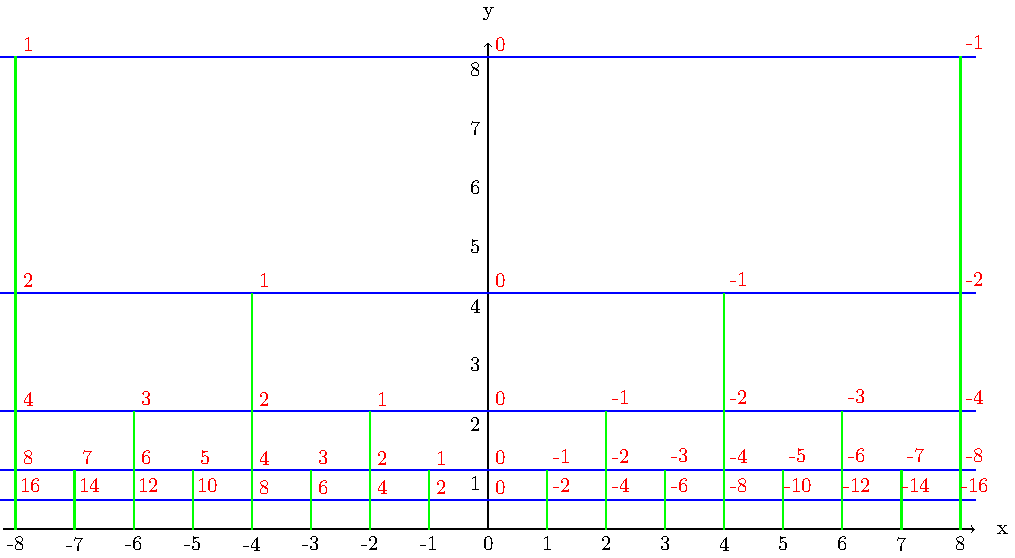
\includegraphics{01-grid-example-1.pdf}}
    \caption{Addition-multiplication grid generated by $+ 1$ and $\times 2$ on the upper half-plane $\mathcal{H}$,
        with red values indicating the assignment field $a = -x/y$.}\label{fig:gridex0}
\end{figure}

On the scalar field $\mathcal{H}$, we construct a grid as illustrated in Figure~\ref{fig:gridex0}.

This grid consists of two orthogonal families of lines, represented by blue and green colors. The red values at intersection points denote the values of the assignment field $a$. The blue lines represent an increment by $+1$ in the assignment field $a$, while the green lines signify a multiplication by $2$.

Arithmetic expressions can be effectively represented as paths on the constructed grid, as demonstrated in Figure~\ref{fig:encoding}.This figure illustrates the encoding of the arithmetic expression $((((1 \times 4) - 1) \times 2) - 3)$ using bold black lines.

\begin{figure}[ht]
\centering
\resizebox{0.9\textwidth}{!}{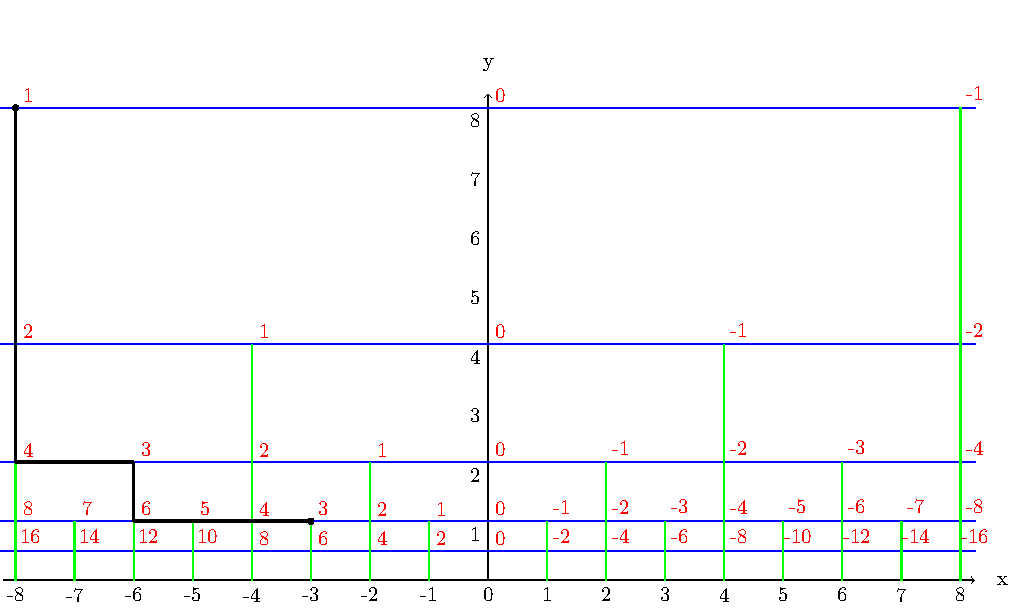
\includegraphics{05-example-expression-embedding}}
\caption{Visualization of encoding a threadlike expression}\label{fig:encoding}
\end{figure}

The depicted zigzag path in Figure~\ref{fig:encoding} is decomposed into four segments, each corresponding to specific arithmetic operations:
\begin{itemize}
\item A vertical segment ascending from $1$ to $4$, representing a multiplication by $4$. This segment corresponds to traversing two steps along the multiplicative axis of the grid.
\item A horizontal segment from $4$ to $3$, signifying a subtraction by $1$. This segment represents a single step along the additive axis.
\item Another vertical segment from $3$ to $6$, indicating a multiplication by $2$, involving one step upward along the multiplicative axis.
\item The final horizontal segment from $6$ to $3$, representing a subtraction by $3$, covering three steps along the additive axis.
\end{itemize}

This encoding method provides a clear and systematic representation of arithmetic operations within a geometric framework, allowing for an intuitive visualization of complex expressions.

In a similar fashion, Figure~\ref{fig:canonicalform} presents various paths and their associated expressions, all originating from the source $1$ and converging at the same target, $3$. These expressions serve as a means of evaluating arithmetic operations in a consistent, lineage-based manner, aptly termed threadlike expressions. The illustrated paths also represent diverse encoding strategies within a canonical framework:

\begin{itemize}
    \item The \textbf{black path} represents the expression $((1 \times 8) - 5) = 3$.
    \item The \textbf{purple path} encodes $((1 - \frac{5}{8}) \times 8) = 3$.
    \item The \textbf{brown path} is detailed as $((((((1 - \frac{1}{8}) \times 2) - \frac{1}{2}) \times 2) - 1) \times 2) = 3$.
    \item The \textbf{orange path} encompasses infinitely many addition-multiplication terms, representing a specialized form of integration.
\end{itemize}

\begin{figure}[ht]
\centering
\resizebox{0.9\textwidth}{!}{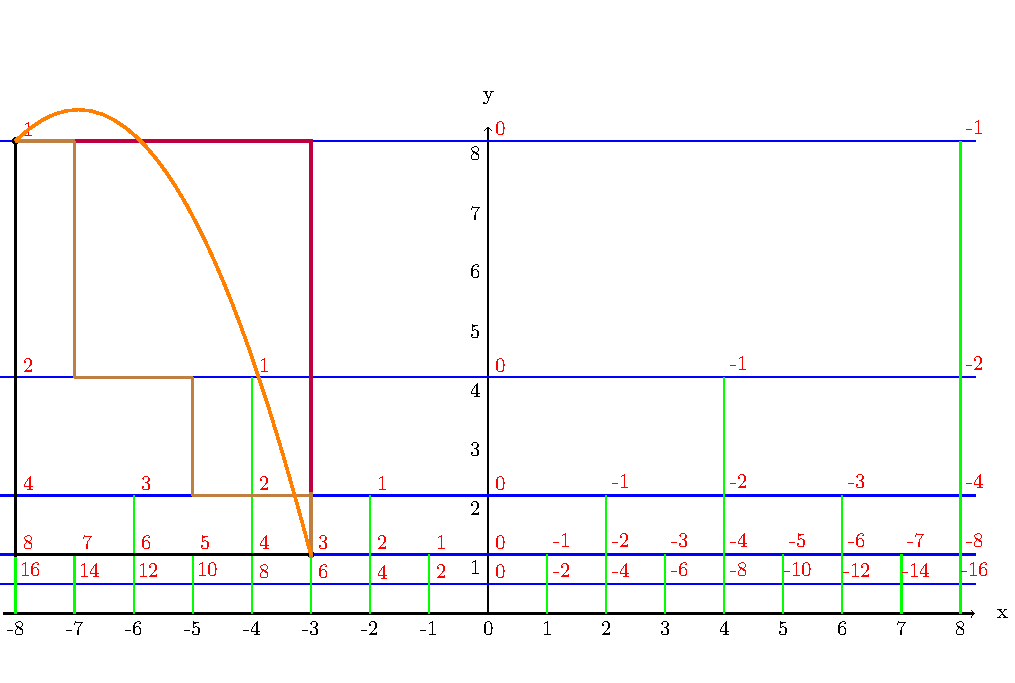
\includegraphics{06-example-canonical-form}}
\caption{Illustration of different encodings and their canonical forms}\label{fig:canonicalform}
\end{figure}

These paths not only share common endpoints but also demonstrate how arithmetic expressions can be algebraically
manipulated to transform one into another through the application of the distributive law and
by methodically combining and decomposing terms.

Transformation from the brown path to the black path:
\begin{align}
    3 & = ((((((1 - \frac{1}{8}) \times 2) - \frac{1}{2}) \times 2) - 1) \times 2) \\
    & = 1 \times 8 -  \frac{1}{8} \times 8 - \frac{1}{2} \times 4 - 1 \times 2 \\
    & = ((1 \times 8) - 5)
\end{align}

Transformation from the brown path to the purple path:
\begin{align}
    3 & = ((((((1 - \frac{1}{8}) \times 2) - \frac{1}{2}) \times 2) - 1) \times 2) \\
    & = (1 - \frac{1}{8}) \times 8 - \frac{1}{2} \times 4 - 1 \times 2 \\
    & = (1 - \frac{1}{8}) \times 8 - \frac{1}{4} \times 8 -  \frac{1}{4} \times 8 \\
    & = (1 - \frac{1}{8} - \frac{1}{4} - \frac{1}{4}) \times 8 \\
    & = ((1 - \frac{5}{8}) \times 8)
\end{align}

Consequently, the black and purple paths depicted in Figure~\ref{fig:canonicalform} can be designated as canonical paths. These paths exemplify all possible threadlike expressions that connect the initial point, represented by the source $1$, to the terminal point, $3$.

With the establishment of such canonical paths, any arbitrary target point $P$ can be systematically related to a predetermined source point $O$ through a canonical path. This structured approach permits the conceptualization of the entire domain as a collection of canonical expressions. Thus, we define this domain explicitly as a space of expressions, where each point connection adheres to a canonical form.

\section{Basic concepts}\label{sec:concepts}

\subsection{Arithmetic expression}\label{sec:expression}

In order to define arithmetic expressions involving real numbers  $\mathbb{R}$ in a rigorous way, we need to use a sophisticated type theory. However, in order to keep things simple and maintain clarity, we will start by using only production rules, but with certain semantic restrictions. We will also begin with rational numbers $\mathbb{Q}$ to avoid the difficulties inside real numbers $\mathbb{R}$ .

\begin{definition}\label{def:arithmetic-expression}
An arithmetic expression $a$ over $\mathbb{Q}$ is a structure given by the following production rules:
\begin{equation}\label{eq:productionrule}
\begin{aligned}
    a &\longleftarrow x\\
    a &\longleftarrow ( a + a )\\
    a &\longleftarrow ( a - a )\\
    a &\longleftarrow ( a \times a )\\
    a &\longleftarrow ( a \div a )
\end{aligned}
\end{equation}
where $x \in \mathbb{Q}$, and we denote this as $a \in \mathbb{E} \left [\mathbb{Q} \right ]$.
\end{definition}

During the production process, we can obtain both a string representation and a tree representation of arithmetic expression $a$,
where the two representations are equivalent.
For instance, the string representation of $a$ might be:

\begin{equation}
    (((((1 \times 2) \times 2) - 1) \times (2 + 1)) - 6)\label{eq:equation}
\end{equation}

and the parsed syntax tree is depicted in Figure~\ref{fig:syntaxtree}.

\begin{figure}[ht]
    \centering
    \resizebox{0.2\textheight}{!}{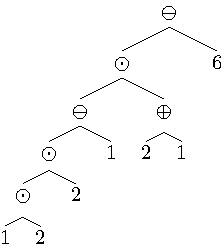
\includegraphics{02-example-expression-syntax-tree.pdf}}
    \caption{a tree representation of an arithmetic expression}\label{fig:syntaxtree}\label{fig:figure}
\end{figure}

If we interpret the target as a string and the building processes in production rule~\eqref{eq:productionrule} as string building, we get the \emph{string representation}.
On the other hand, if the target is a tree, tree building leads to the \emph{tree representation}.
We can easily obtain the string representation of $a$ from its tree representation by performing a pre-order traversal.

The concept of a \emph{sub-expression} can also be derived from the concept of a subtree.
The branch nodes are all labeled with operators: $+$, $-$, $\times$, $\div$.
The leaf nodes are all labeled with numbers.

Evaluation $\nu$ is a partial function that operates on arithmetic expression $a \in \mathbb{E} \left [\mathbb{Q} \right ]$.
It is undefined only if division by zero occurs during the recursive evaluation process.

We can define evaluation $\nu(a)$ of $a$ recursively as follows:
\begin{itemize}
    \item Constant leaf: For any $x \in \mathbb{Q}$, $\nu(x) = x$.
    \item Compositional node by $+$: For any $(a + b)$, $\nu((a + b)) = \nu(a) + \nu(b)$.
    \item Compositional node by $-$: For any $(a - b)$, $\nu((a - b)) = \nu(a) - \nu(b)$.
    \item Compositional node by $\times$: For any $(a \times b)$, $\nu((a \times b)) = \nu(a) \nu(b)$.
    \item Compositional node by $\div$: For any $(a \div b)$, if $\nu(b) \neq 0$, then $\nu((a \div b)) = \nu(a) / \nu(b)$.
\end{itemize}

We say that an arithmetic expression $a$ is \emph{evaluable} if $\nu(a)$ is defined.
In the rest of this article, we will only consider evaluable arithmetic expressions unless stated otherwise.

Given an arithmetic expression $a$, whatever evaluable or not, we can obtain its tree representation.
If a node $l$ is a leaf node, its corresponding subexpression $s$ is a number, so we consider it to be already \("\)evaluated\("\).
If a node $b$ is a branch node, its corresponding subexpression $s$ is an expression, and we can apply $\nu$ to it to obtain a number $\nu(s)$.
During the recursive evaluation process, starting from the leaves and moving towards the root, the subexpressions are evaluated one after another.
However, the order of evaluations is generally not unique.

\begin{definition}
    The evaluation order of an arithmetic expression $a$ is an ordering of branch nodes in the tree representation of $a$
    such that every node (sub-expression) is evaluated before its parent.
\end{definition}

For example, the possible evaluation orders of the arithmetic expression in Figure~\ref{fig:syntaxtree} are:
\begin{itemize}
    \item $1 \times 2 \rightarrow \underline{2}; \underline{2} \times 2 \rightarrow \underline{4}; \underline{4} - 1 \rightarrow \underline{3}; 2 + 1 \rightarrow \underline{3}; \underline{3} \times \underline{3} \rightarrow \underline{9}; \underline{9} - 6 \rightarrow 3$
    \item $1 \times 2 \rightarrow \underline{2}; \underline{2} \times 2 \rightarrow \underline{4}; 2 + 1 \rightarrow \underline{3}; \underline{4} - 1 \rightarrow \underline{3}; \underline{3} \times \underline{3} \rightarrow \underline{9}; \underline{9} - 6 \rightarrow 3$
    \item $1 \times 2 \rightarrow \underline{2}; 2 + 1 \rightarrow \underline{3}; \underline{2} \times 2 \rightarrow \underline{4}; \underline{4} - 1 \rightarrow \underline{3}; \underline{3} \times \underline{3} \rightarrow \underline{9}; \underline{9} - 6 \rightarrow 3$
    \item $2 + 1 \rightarrow \underline{3}; 1 \times 2 \rightarrow \underline{2}; \underline{2} \times 2 \rightarrow \underline{4}; \underline{4} - 1 \rightarrow \underline{3}; \underline{3} \times \underline{3} \rightarrow \underline{9}; \underline{9} - 6 \rightarrow 3$
\end{itemize}

The underlined numbers are the numbers that are evaluated during the evaluation process.

Below are examples of expressions that have a unique evaluation order.
These include right-expanded, left-expanded,
and combinations of them, as shown in Figure~\ref{fig:leftright} and Figure~\ref{fig:combination}.

\begin{figure}[ht]
    \centering
    \resizebox{0.4\textheight}{!}{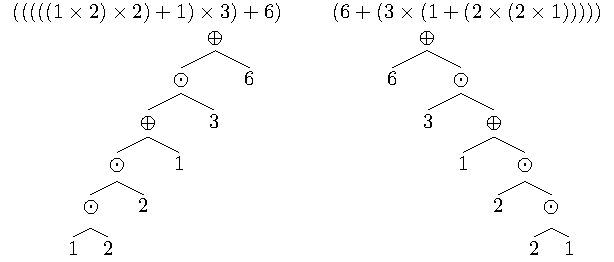
\includegraphics{03-example-expression-syntax-tree-left-right.pdf}}
    \caption{right-expanded and left-expanded expressions}\label{fig:leftright}
\end{figure}

\begin{figure}[ht]
    \centering
    \resizebox{0.2\textheight}{!}{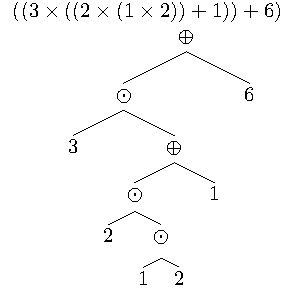
\includegraphics{04-example-expression-syntax-tree-combination}}
    \caption{combinations of right-expanded and left-expanded expressions}\label{fig:combination}
\end{figure}

The evaluation order of an arithmetic expression is related to the topological order of its tree representation, but they are not the same.
The topological order of a tree is an ordering of nodes such that every node is visited before its parent\cite{Knuth1997TheAO}.
However, we are only interested in the ordering of branch nodes, as leaf nodes have already been evaluated and can be ignored.
Additionally, the topological order goes from parent to children, while the evaluation order goes from children to parent.

\begin{definition}
    A threadlike expression is an arithmetic expression that all the left nodes in its tree representation are leaf nodes.
\end{definition}

So a threadlike expression is right-expanded and its evaluation order is unique.
One example of threadlike expressions is shown on the left side of Figure~\ref{fig:leftright}.

Threadlike expressions are significant here because they are analogous to the concept of paths in homotopy theory in geometry.
In a more general context, certain special types of threadlike expressions are also interesting:
for example, \emph{alternating threadlike expressions} are expressions in which the additional and multiplicative operators appear in an alternating manner.
In the field of computing, a hardware component called \emph{multiplier-accumulator} (MAC) unit has been implemented~\cite{Quinnell2007FloatingPointFM},
which is a special case of an alternating threadlike expression.
As a result, some numerical algorithms based on MAC units have been studied~\cite{Markstein2004SoftwareDA}.

\subsection{Currying and path notation}\label{subsec:currying}

Currying is a basic technique in functional programming\cite{Reynolds1972DefinitionalIF},
which is used to transform a function with multiple arguments into a sequence of functions with one argument.
By currying a threadlike arithmetic expression, we can obtain a sequence of functions that operate on an operand, which is the leftmost leaf node.

We introduce the following notation for currying a threadlike arithmetic expression:
\begin{itemize}
    \item initial operand: the leftmost leaf node
    \item operator: $\oplus_y: x \mapsto x + y$
    \item operator: $\ominus_y: x \mapsto x - y$
    \item operator: $\otimes_y: x \mapsto x \cdot e^y$
    \item operator: $\oslash_y: x \mapsto x \cdot e^{-y}$
\end{itemize}

For example, the threadlike arithmetic expression $(((((1 \times 2) \times 2) + 1) \times 3) + 6)$ can be curried as

\[\oplus_6(\otimes_{\ln 3}(\oplus_1(\otimes_{\ln 2}(\otimes_{\ln 2}(1)))))\]

Suppose we have a series of operators $a_1, a_2, \cdots a_{n-1}, a_n$, we introduce a \emph{path notation}.

\[x a_1 a_2 \cdots a_{n-1} a_n \coloneqq a\_n( a_{n-1}( \cdots a_2( a_1(x) ) \cdots ) )\]

So, the above example can be written as

\[1 \otimes_{\ln 2} \otimes_{\ln 2} \oplus_1 \otimes_{\ln 3} \oplus_6 \]

If a path begins with a number, we refer to it as a \emph{bounded path}.
If it does not, we refer to it as a \emph{free path}, similar to the concept of vectors from the origin versus vectors at arbitrary points.
a bounded path results in a number, while a free path results in a function.

Now we will verify that the operators within a path are associative.

\begin{lemma}\label{lemma:associative}
The operators within a path are associative, i.e. we have \[a [b c] = [a b] c\]
\end{lemma}

\begin{proof}
    We use normal typeface to express the path notation, and bold typeface to express the function notation.

    For a free path, follow the definition, we have
    \[a [b c] = [b c](\mathbf{a}) = \mathbf{c}(\mathbf{b}(\mathbf{a}))\]
    \[[a b] c = \mathbf{c}([a b]) = \mathbf{c}(\mathbf{b}(\mathbf{a}))\]

    hence, we have
    \[a [b c] = [a b] c\]
    is hold for a free path.

    For a bounded path, we have
    \[x a [b c] = [b c](\mathbf{a}(x)) = \mathbf{c}(\mathbf{b}(\mathbf{a}(x)))\]
    \[x [a b] c = \mathbf{c}([a b](x)) = \mathbf{c}(\mathbf{b}(\mathbf{a}(x)))\]

    hence, we have
    \[a [b c] = [a b] c\]
    is hold for a bounded path.

\end{proof}

\begin{definition}\label{definition:concatenate}
The concatenation of paths $p_1 \cdot p_2$ is defined as the composite of functions:
\[p_1 \cdot p_2 \coloneqq p_2 \circ p_1 \]
\end{definition}

When a sequence of paths is concatenated, and only the first path can be bounded.
If the first path is bounded, the concatenated result is a bounded path.
Otherwise, the concatenated result is a free path.

\subsection{Alternating threadlike expressions}\label{subsec:alternating}

Now we can define alternating threadlike expressions, which were mentioned in Section~\ref{sec:expression}, using the path notion.

\begin{equation}\label{eq:alternative}
\alpha = a_1 b_1 a_2 b_2 \cdots a_l b_l, a_i = \otimes_{\lambda_i}, b_i = \oplus_{\mu_i}, \lambda_i, \mu_i \in \mathbb{R}
\end{equation}

where $\bigoplus$ and $\bigotimes$ denote addition and multiplication, respectively,
and the expression is a zigzag of alternating addition and multiplication operations.
$\alpha$ is a free path, and we can bind a number to it.

Since $0$ is the identity element for addition and $1$ is the identity element for multiplication,
it is straightforward to see that any arithmetic expression can be converted into an alternating threadlike expression
by introducing more $0$ and $1$ into the original expression.
So alternating threadlike expression is a kind of canonical form.

We can derive a formula for perturbations in alternating threadlike expressions.

Let us define the left-to-right accumulated sum of $\lambda_i$ as $\check{\lambda}_i$, such that:
\begin{equation}
    \check{\lambda}_i = \sum_{j=1}^i \lambda_j, \check{\lambda}_0 = 0\label{eq:accsumlr}
\end{equation}

Then we also have right-to-left accumulated sum of $\lambda_i$
\begin{equation}
    \hat{\lambda}_i = \check{\lambda}_l - \check{\lambda}_{l - i}, \hat{\lambda}_0 = 0\label{eq:accsumrl}
\end{equation}

Expanding equation~\eqref{eq:alternative} using the distributive law and the above notion at point $\mu_0$, we obtain:
\begin{align}
    \alpha(\mu_0) & = e^{\lambda_l}(\cdots (e^{\lambda_2} (e^{\lambda_1} \mu_0 + \mu_1) + \mu_2) \cdots) + \mu_l \\
    & = e^{\hat{\lambda}_l} \mu_0 + e^{\hat{\lambda}_{l - 1}} \mu_1  + e^{\hat{\lambda}_{l - 2}} \mu_2 + \cdots + e^{\hat{\lambda}_1} \mu_{l - 1} + e^{\hat{\lambda}_0} \mu_l
\end{align}

Next, at the starting point $\mu_0$, we introduce a perturbation $\tilde{\mu}_0 = e^{\eta_0} \mu_0 + \epsilon_0$,
where $\eta_0$ and $\epsilon_0$ are the disturbance terms added by the summation and multiplication operations, respectively. Then, we have:
\begin{align}
    \alpha(\tilde{\mu}_0) & = e^{\hat{\lambda}_l} (\tilde{\mu}_0) + e^{\hat{\lambda}_{l - 1}} \mu_1  + e^{\hat{\lambda}_{l - 2}} \mu_2 + \cdots + e^{\hat{\lambda}_1} \mu_{l - 1} + e^{\hat{\lambda}_0} \mu_l \\
    & = \alpha(\mu_0) + e^{\hat{\lambda}_l} (\tilde{\mu}_0 - \mu_0)
\end{align}

As a result, purely from an arithmetic perspective, without the need for limits, we can derive the following meaningful ratio:
\begin{equation}
    \frac{\alpha(\tilde{\mu}_0) - \alpha(\mu_0)}{\tilde{\mu}_0 - \mu_0} = e^{\hat{\lambda}_l} = e^{\check{\lambda}_l}\label{eq:ratio}
\end{equation}

Now we extend this relationship from the starting point $\mu_0$ to the entire process, we define the recursive formula

\[
    w_i = e^{\lambda_i} w_{i-1} + \mu_i, w_0 = 0
\]

and then we have

\begin{equation}
    \frac{\tilde{w}_i - w_i}{\tilde{\mu}_0 - \mu_0} = e^{\check{\lambda}_i}, i \in \{1, ..., l\}\label{eq:perturbation1}
\end{equation}

So, we have

\[
    \tilde{w}_i - w_i = e^{\check{\lambda}_i} (\tilde{\mu}_0 - \mu_0)
\]

and hence

\begin{equation}
    \tilde{w}_i - w_i = e^{\lambda_i}(\tilde{w}_{i - 1} - w_{i - 1})\label{eq:perturbation2}
\end{equation}

That means the perturbation along the path is controlled by the multiplication terms of $e^{\lambda_i}$.

\subsection{Generated structure, commutator and arithmetic torsion}\label{subsec:generated-structure}

In order to study mesh grids like the one described in section~\ref{sec:example},
we need to investigate the algebraic structure of the threadlike arithmetic expressions that are generated.

For real number $\mathbb{R}$ and elements $\mu, \lambda \in \mathbb{R}$, we consider all the arithmetical expressions
that are freely generated from
\begin{itemize}
    \item initial operand: $0$
    \item operator: $\oplus_\mu: x \mapsto x + \mu$
    \item operator: $\ominus_\mu: x \mapsto x - \mu$
    \item operator: $\otimes_\lambda: x \mapsto x \cdot e^\lambda$
    \item operator: $\oslash_\lambda: x \mapsto x \cdot e^{- \lambda}$
\end{itemize}

We denote these expressions as $E(\mu, \lambda)$, where $\mu$ is the additional generator and $e^\lambda$ is the multiplicative generator.
In cases where the context is clear, we may omit $\mu$ and $\lambda$ from the index.
Our goal is not to study only a single $E(\mu, \lambda)$, but rather to use a family of $E(\mu, \lambda)$ to approach a continuous space.

Since $\oplus_\mu$ and $\ominus_\mu$ are mutually inverse operations, it follows that $\otimes_\lambda$ and $\oslash_\lambda$ are also mutually inverse. This means that $E(\mu, \lambda)$ forms a group.
An observation is that the commutator of this group is not equal to identity generally,
especially the commutator of the generators.

\begin{equation}
    x \oplus_\mu \otimes_\lambda \ominus_\mu \oslash_\lambda - x = \mu(1 - e^{-\lambda})\label{eq:commutator1}
\end{equation}
\begin{equation}
    x \otimes_\lambda \oplus_\mu \oslash_\lambda \ominus_\mu - x = - \mu(1 - e^{-\lambda})\label{eq:commutator2}
\end{equation}

Formula \ref{eq:commutator1} obey the right-hand rule, and formula \ref{eq:commutator2} obey the left-hand rule.

Or equivlently, we define below difference $\tau$ obey the right-hand rule:

\begin{equation}
    \tau = x \oplus_\mu \otimes_\lambda - x \otimes_\lambda \oplus_\mu = \mu(e^\lambda - 1)\label{eq:torsion}
\end{equation}

These differences are constant, indicating a type of torsion in the generated group.
And torsion $\tau$ is specifically referred to as the arithmetic torsion.

\section{Flow equation}\label{sec:flowequation}

\subsection{Flow equation}\label{sec:equation}

Consider an infinitesimal generating process on a Riemannian surface $M$ using two generators:
one for an additional action $\mu$ and the other for a multiplicative action $e^\lambda$.
These two generators are perpendicular.
This generation process produces an assignment $A: M \to R$ over the surface.

For any point with an assignment $a_0$, if we consider a movement of distance $\epsilon$ in a direction with angle $\theta$
over a time period of $\delta$, we can establish the following:

\[
    a_{\delta} = (a_0 + \mu \epsilon \cos \theta)e^{\lambda \epsilon \sin \theta}
\]

or

\[
    a_{\delta} = a_0 e^{\lambda \epsilon \sin \theta} + \mu \epsilon \cos \theta
\]

Both formula can be simplified to the same result:

\[
    a_{\delta} = a_0 + \epsilon (a_0 \lambda \sin \theta + \mu \cos \theta)
\]

Then, we have the following equation:

\[
    \frac{1}{\delta} (a_{\delta} - a_0) = \frac{\epsilon}{\delta} (\mu \cos \theta + x_0 \lambda \sin \theta)
\]

When both $\delta$ and $\epsilon$ are towards zero, we get $da / dt$, and hence

\[
    \frac{da}{dt} = u (\mu \cos \theta + a \lambda \sin \theta)
\]

Or, we can change it to another form

\begin{equation}
    \frac{da}{ds} = \mu \cos \theta + a \lambda \sin \theta\label{eq:flow}
\end{equation}

We name this equation~\eqref{eq:flow} as the flow equation.

We can also get a direct formal solution of the flow equation~\eqref{eq:flow}(details in Appendix~\ref{sec:directformalsolution}).

\begin{equation}
    a = (a_0 + \frac{\mu}{\lambda} \cot \theta) e^{\lambda s \sin \theta} - \frac{\mu}{\lambda} \cot \theta\label{eq:solution}
\end{equation}

\subsection{Discrete generating}\label{subsec:discrete-generating}

In section~\ref{subsec:generated-structure}, we have discussed a discrete generating process.
Since flow equation governs an infinitesimal generating process,
we will show the above discrete generating process can be emerged from the solution of the flow equation~\eqref{eq:solution} naturally.
We expand the formula by the Taylor series:

\[
    a =  a_0 e^{\lambda s \sin \theta} + \frac{\mu}{\lambda} [1 + \lambda s \sin \theta + \frac{1}{2!} (\lambda s \sin \theta)^2  + \frac{1}{3!} (\lambda s \sin \theta)^3 + \cdots - 1] \cot \theta
\]

Change the formula slightly:
\[
    a = a_0 e^{\lambda s \sin \theta} + \mu s \cos \theta + \frac{\mu}{\lambda} \sin \theta \cos \theta (\frac{\lambda^2s^2}{2!} + \frac{\lambda^3s^3}{3!} \sin \theta + \frac{\lambda^4s^4}{4!} \sin^2 \theta + \cdots)
\]

By the formula of double angle, we have
\[
    a = a_0 e^{\lambda s \sin \theta} + \mu s \cos \theta + \frac{\mu}{2\lambda} \sin 2\theta (\frac{\lambda^2s^2}{2!} + \frac{\lambda^3s^3}{3!} \sin \theta + \frac{\lambda^4s^4}{4!} \sin^2 \theta + \cdots)
\]

We denote
\begin{equation}
    \Psi(s) = \frac{1}{2!} + \frac{\lambda s}{3!} \sin \theta + \frac{\lambda^2 s^2}{4!} \sin^2 \theta + \cdots
\end{equation}

Then we have
\begin{equation}
    a = a_0 e^{\lambda s \sin \theta} + \mu s \cos \theta + \frac{\mu\lambda}{2} s^2 \Psi(s) \sin 2\theta
\end{equation}

This formula gives the discrete generating process, when $\theta = \frac{k \pi}{2}, k = 0, 1, 2, 3\cdots, s = 0, 1, 2, 3\cdots$, we have

\begin{equation}
    a = a_0 e^{\lambda s \sin \theta} + \mu s \cos \theta
\end{equation}

Especially, we have the following four cases:
\begin{itemize}
    \item $\theta = 0$: $a_s = a_0 + \mu s$
    \item $\theta = \frac{\pi}{2}$: $a_s = a_0 e^{\lambda s}$
    \item $\theta = \pi$: $a_s = a_0 - \mu s$
    \item $\theta = \frac{3 \pi}{2}$: $a_s = a_0 e^{- \lambda s} $
\end{itemize}

This result is straightforward, but it demonstrates that the infinitesimal generating process is consistent with the discrete generating process.
And this expands our toolset, enabling us to explore the interplay between discrete and infinitesimal generating processes.

\subsection{The contour-gradient form of flow equation}\label{subsec:the-contour-gradient-form}

It is easy to derive the contour equation in the local coordinate

\begin{equation}
    \mu \cos \theta_c + a \lambda \sin \theta_c = 0\label{eq:contour}
\end{equation}

then we have

\begin{equation}
    \theta_c = - \arctan \frac{\mu}{a \lambda}\label{eq:contourangle}
\end{equation}

the contour and the gradient are perpendicular to each other

\begin{equation}
    \theta_g = \pm \frac{\pi}{2} - \arctan \frac{\mu}{a \lambda}\label{eq:gradientangle}
\end{equation}

then along $\theta_g$ we have

\begin{equation}
    \frac{da}{ds} = \mu \cos (\pm \frac{\pi}{2} - \arctan \frac{\mu}{a \lambda}) + a \lambda \sin (\pm \frac{\pi}{2} - \arctan \frac{\mu}{a \lambda})
    \label{eq:alonggradient}
\end{equation}

\begin{equation}
    \frac{da}{ds} = \pm \sqrt{\mu^2 + \lambda^2 a^2}\label{eq:grad}
\end{equation}

By introducing the right-hand rotation angle $\phi$ along the gradient direction, we can establish a local polar coordinate system based on the gradient and contour lines.
Then the growth rate of $a$ along the angle $\phi$ is

\begin{equation}
    \frac{da}{ds} = \mu \cos (\frac{\pi}{2} - \arctan \frac{\mu}{a \lambda} + \phi) + a \lambda \sin (\frac{\pi}{2} - \arctan \frac{\mu}{a \lambda} + \phi)
    \label{eq:fourfold}
\end{equation}

And the simplified equation is

\begin{equation}
    \frac{da}{ds} = \sqrt {\mu^2 + a^2 \lambda^2} \cos \phi\label{eq:contourgradient}
\end{equation}

or

\begin{equation}
    \frac{da_{\phi}}{ds_{\phi}} = \sqrt {\mu^2 + a^2 \lambda^2} \cos \phi\label{eq:contourgradient2}
\end{equation}

if we want to emphasize the path is along the angle $\phi$.

The equation~\eqref{eq:contourgradient} is the flow equation in the contour-gradient coordinate system.

Equation~\eqref{eq:contourgradient} is solvable, and we get the relation between $a$ and $s$:

\begin{equation}\label{eq:rel_a_s}
\tanh(\lambda s \cos \phi - c) = \frac{\lambda a}{\sqrt{\mu^2 + \lambda^2 a^2}}
\end{equation}

we can further simplify the equation to

\begin{equation}
    a = \pm \frac{\mu}{\lambda} \sinh(\lambda s \cos \phi - c)\label{eq:gradevo}
\end{equation}

Under the initial condition $a = a_0$ when $s = 0$, we can get the following equation:

\begin{equation}
    a = \frac{\mu}{\lambda} \sinh(\lambda s \cos \phi + \arcsinh \frac{a_0 \lambda}{\mu})\label{eq:gradevo2}
\end{equation}

or

\begin{equation}
    a = - \frac{\mu}{\lambda} \sinh(\lambda s \cos \phi - \arcsinh \frac{a_0 \lambda}{\mu})\label{eq:gradevo3}
\end{equation}

In this coordinate system, the additional line and the multiplicative line are:

\begin{equation}
    \phi = \arccos \frac{\mu}{\sqrt {\mu^2 + a^2 \lambda^2}} \label{eq:additionalline}
\end{equation}

\begin{equation}
    \phi = \arcsin \frac{\mu}{\sqrt {\mu^2 + a^2 \lambda^2}}\label {eq:mulitiplcativeline}
\end{equation}

\subsection{Local Descartes coordinate and area formula}\label{subsec:descartes-coordinate}
We begin our exploration by examining the flow equation~\eqref{eq:flow} within the framework of a local polar coordinate system:

\begin{equation}
    \frac{da}{ds} = \mu \cos \theta + a \lambda \sin \theta
\end{equation}

In an effort to re-contextualize this equation, we set $du = \cos \theta ds$ and $dv = \sin \theta ds$,
where $du$ and $dv$ are perpendicular infinitesimal movements.
We can use these movements to construct a local Descartes coordinate system, and the first fundamental form of this system is:

\begin{equation}
    ds^2 = A^2 du^2 + B^2 dv^2
\end{equation}

Thereby this enables us to express the flow equation in a different light:

\begin{equation}
    da = \mu du + a \lambda dv
\end{equation}

or in a partial differential form:

\begin{equation}
    \frac{\partial a}{\partial u} = \mu
\end{equation}

\begin{equation}
    \frac{\partial a}{\partial v} = a \lambda
\end{equation}

Our attention now turns to the concept of arithmetic torsion, particularly at an infinitesimal level.
Delving into the interplay between two infinitesimal generating processes, we observe that:

\begin{equation}
    d\tau = (a_0 + \mu du) e^{\lambda dv} - (a_0 e^{\lambda dv} + \mu du)
\end{equation}

From this relationship, we deduce:

\begin{equation}
    d\tau = \mu du (e^{\lambda dv} - 1)
\end{equation}

This leads us to an area formula, capturing the essence of this interaction:

\begin{equation}
    d\tau = \mu \lambda du dv \label{eq:area_formula}
\end{equation}

and because the area element have a form

\begin{equation}
    dS = |AB| du dv \label{eq:area_element}
\end{equation}

Then we have
\begin{equation}
    \frac{d\tau}{\mu \lambda} = \frac{dS}{|AB|}\label{eq:area_formula2}
\end{equation}

This formula is compelling as it establishes a link between area elements and arithmetic torsion.
It's noteworthy to emphasize the distinctiveness of the local Descartes coordinate system.
This system, by integrating the assignment, lays the foundation for a theoretical framework.
We refer to this as the arithmetic coordinate system, given its unique properties and alignment with arithmetic principles.
The proof of its existence and further elaboration will be undertaken in the upcoming section\ref{subsec:existence-theorems},
underscoring its significance and application in our study.

\section{Arithmetic expression space}\label{sec:space}

\subsection{The definition}\label{subsec:definition}

In the light of previous sections, we introduce a new mathematical object $\mathfrak{E}$, an arithmetic expression space,
as a tuple of $(M, a)$:

\begin{itemize}
    \item $M$: a Riemannian surface
    \item $a$: a smooth assignment function from $M$ to $F$ which satisfied the flow equation.
\end{itemize}

And then we can interpret a smooth path by the flow equation as a threadlike arithmetic expression.

\subsection{Examples}\label{subsec:example}

\emph{Example 1}:

The hyperbolic space equipped with the following metric and assignment in the upper half plane model is an arithmetic expression space.
\[
    ds^2 = \frac{1}{y^2}(\frac{dx^2}{\mu^2} + \frac{dy^2}{\lambda^2})
\]
and assignment
\[
    a = - \frac{x}{y}
\]

The flow equation is satisfied.

\emph{Example 2}:

The hyperbolic space equipped with the following metric and assignment in the horocycle coordinate is an arithmetic expression space.
\[
    ds^2 = e^{-2v} du^2 + dv^2
\]
and assignment
\[
    a = u e^ {-v}
\]

The flow equation is satisfied.

Example 1 and Example 2 are the same assignment field but with different coordinate systems.

\emph{Example 3}:

The hyperbolic space equipped with the following metric and assignment in the Poincaré disk model is an arithmetic expression space.

\[
    ds^2 = dr^2 + \sinh^2 r d\theta^2
\]

and assignment

\[
    a = (e^{2 \arctanh r \sin \theta} -  1) \cot \theta
\]

\subsection{The local existence theorem}\label{subsec:existence-theorems}

There are two existence propositions related to the flow equation~\eqref{eq:flow}.

The first existence propositions states that if we have a Riemannian surface $S$, then there exists a function $a$ on $S$ that satisfies the flow equation~\eqref{eq:flow}.

\begin{proposition}
    Given a Riemannian surface $S$, there exists a function $a$ on $S$ satisfying the flow equation~\eqref{eq:flow}.
    \label{prop:existence1st}
\end{proposition}

The second existence propositions is also interesting.
It says that if we have a smooth surface $S$ and a function $a$ on $S$, then we can find a metric $g$ on $S$ that makes $a$ satisfy the flow equation~\eqref{eq:flow}.
We morph the metric $g$ to make $a$ satisfy the flow equation~\eqref{eq:flow}.

And we had proved a local version of the second existence propositions as a theorem.
\begin{theorem}(By Le Zhang)
    For every point \( p \) on an oriented compact Riemannian surface $S$, and a smooth function $a$ over $S$, there exists a metric $g$ on a neighborhood surrounding \( p \)
    that makes $a$ satisfying the flow equation~\eqref{eq:flow}.
    \label{prop:existence2nd}
\end{theorem}

\begin{proof}
    Consider a neighborhood \( U \) around \( p \).
    In this area, we can find a local isothermal coordinate system in which the metric takes the form:
    \[ ds^2 = e^{2\rho}(du^2 + dv^2), \]
    where \( u \) and \( v \) are the coordinates of \( U \), and \( \rho \) is a function of \( u, v \) in \( U \).
    The gradient of \( a \) in this local isothermal coordinate system is expressed as:
    \[ \nabla a = \frac{\partial a}{\partial u} du + \frac{\partial a}{\partial v} dv. \]
    Using the definition of the directional derivative, we obtain:
    \[ \frac{da_{\psi}}{ds_{\psi}} = ||\nabla a|| \cos \psi, \]
    where \( ||\nabla a|| \) is the norm of \( \nabla a \), and \( \psi \) is the angle between \( \nabla a \) and the direction of movement.

    Now, considering the flow equation~\ref{eq:contourgradient2} in the gradient-contour coordinate system, we have:
    \[ \frac{da_{\phi}}{ds_{\phi}} = \sqrt{\mu^2 + a^2 \lambda^2} \cos \phi. \]

    Note that \( ||\nabla a|| \) is fixed for the given function \( a \) and the local coordinate system, and \( \sqrt{\mu^2 + a^2 \lambda^2} \) is also fixed for the given function \( a \).
    We can scale \( e^{2\rho} \) with a linear factor \( \alpha \) to make \( ||\nabla a|| \) match the fixed value of \( \sqrt{\mu^2 + a^2 \lambda^2} \),
    thus we have a morphing process controlled by \( \alpha \) that
    \begin{align}
        ds^2 &= \alpha e^{2 \rho}(du^2 + dv^2)\label{eq:morphing} \\
        &= e^{2 \rho + \ln \alpha}(du^2 + dv^2).
    \end{align}

    Under the morphing ratio \( \alpha \), we have:

    \begin{equation}
        ||\nabla_\alpha a|| = \alpha^{-1} ||\nabla a||,
    \end{equation}

    and when \( \alpha \) is set to the value of:

    \[ ||\nabla_\alpha a|| = \sqrt{\mu^2 + a^2 \lambda^2}, \]

    the flow equation~\eqref{eq:flow} is satisfied in the local coordinate system.

    The morphing ratio \( \alpha \) is calculated as follows:
    \begin{equation}
        \alpha = \frac{||\nabla a||}{\sqrt{\mu^2 + a^2 \lambda^2}}\label{eq:ratio}.
    \end{equation}
    \qedhere

\end{proof}

\section{Conclusion}\label{sec:conclusion}

In this paper, we addressed the existence of a geometry space composed entirely of arithmetic expressions.
We provided a rigorous framework and demonstrated that such a space can indeed be constructed.
Furthermore, we illustrated how the flow equation plays a central role in generating and transforming arithmetic expressions within this constructed geometry.

Our work opens up a new avenue for exploring the interplay between arithmetic and geometry.
We believe that this novel approach will lead to a deeper understanding of the underlying principles in below areas:
\begin{itemize}
    \item Analysis: a new kind of integral which mixes addition and multiplication.
    \item Geometry: a new arithmetic means to study the geometry of surfaces.
    \item Computational complexity: a test bed to study time and space complexity of algorithms in a geometric way.
\end{itemize}

We hope that our work will inspire further research in these areas and provide a fresh perspective on the relationship between arithmetic and geometry.

\bibliographystyle{plain}
\bibliography{main}

\end{document}
